\vspace{2ex}

    {\bf Solution.} I use {\em Stan} platform with {\em PyStan} interface for
    {\em Python programming language}. The problem is that it does not handle
    unbounded discrete parameters. Therefore we use the approach suggested in
    the documentation \cite{stan} considering the population size a continuous
    variable. I tried to use the package {\em PyMC3} for this model (this
    package handles discrete parameters), but given convergence problems,
    I do not present the results. 
    
    \ind As I will present posteriorly, this problem
    may be related to the sampler Metropolis. For the Geometric and
    independent approach, it is possible to compare the analytic curve with
    Stan result (considering $N$ a real variable), and Stan got a well
    approximate result, while PyMC3 had convergence problems. I used 50
    thousand iterations with 5 chains. The parameter adapt delta varied
    between 0.95 and 0.99. 

    \vspace{2ex}

    {\bf Choose of the hyperparameters}

    \vspace{2ex}

    \ind In table \ref{tab:hyperparameters-models}, I presented the hyperparameters
    chosen for the models. Appendix \ref{sec:prior-predictive-checking}, it is
    presented a simple analysis for it. For the Raftery approach, we chose a
    uniform distribution on $\theta$ (given we have no information about the
    populations), and we define the Gamma parameters to have mean and variance
    1. For the uninformative model, we can't make prior analysis since the
    improper choice. For the geometric independent model, we set the
    hyperparameters to have uniform distribution in $(0,1)$. Lastly, the
    parameters in Geometric correlated model have the following
    interpretation: if we want $\theta$ to have mean 0.5, it will have odds 1
    and log-odds 0. The same for $\nu$. We choose the variance to be the value
    such that the prior variance
    of $\nu$ and $\theta$ be around the variance of $\nu$ and $\theta$ in the independent case and a positive correlation of $0.4$, since when the population grows
    (therefore its mean grows, and $\nu$ decreases), we expect $\theta$ to
    decrease (the probability to see a specific individual of the population). 

    \vspace{2ex}

    {\bf Impala data set}

    \vspace{2ex}

    \ind In Figures \ref{fig:marginal-posteriors}, I sketch the marginal posterior
    distributions for each approach. In table \ref{tab:summary-statistics-posterior-impala}, it is
    shown the Bayes estimator under quadratic loss (the expected value
    \cite[Section 4]{Robert2007}), under loss \ref{eq:relative_loss} (MRSE),
    the median point estimate, and 95\%
    highest density interval (HDI).We observe that the shape of
    the posterior distributions are quite similar, with fast grow between
    30-40, and a slow or fast decay, depending on the priors. The more
    uninformative prior we use, the heavier the tail of the distribution. We
    observe the mean is not a robust estimative, while the MRSE changes very
    little. Therefore, the prior modelling is impacted only in the tail. A
    distribution more uninformative generates larger intervals, what is
    expected.

    \vspace{2ex}

    {\bf Waterbuck data set}

    \vspace{2ex}

    \ind In Figures \ref{fig:marginal-posteriors-waterbuck}, I sketch the marginal posterior
    distributions for each approach. In table \ref{tab:summary-statistics-posterior-waterbuck}, it is
    shown the summary statistics. We observe a similar behavior from the
    graphics when compared to the impala data set. The
    uninformative prior generated a much heavier tail, though. 

\begin{table}[!ht]
    \centering
    \begin{tabular}{ccccc}
    \hline
    \textbf{Model}                 & \multicolumn{4}{c}{\textbf{Parameters}}                                                                           \\ \hline
    \textbf{Raftery}               & $\alpha = 1$       & $\beta =1 $      & $a = 1$                                & $b = 1$                              \\
    \textbf{Geometric independent} & $\alpha_1 = 1$     & $\beta_1 = 1$    & $\alpha_2 = 1$                         & $\beta_2 = 1$                        \\
    \textbf{Geometric correlated}  & \multicolumn{2}{c}{$\eta = [0, 0]$} & \multicolumn{2}{c}{$\Sigma = \begin{bmatrix} 2.5 & 1.0 \\ 1.0 & 2.5 \end{bmatrix}$} \\ \hline
    \end{tabular}
    \caption{Hyperparameters for the developed models.}
    \label{tab:hyperparameters-models}
\end{table}

\begin{figure}[ht]
    \centering
    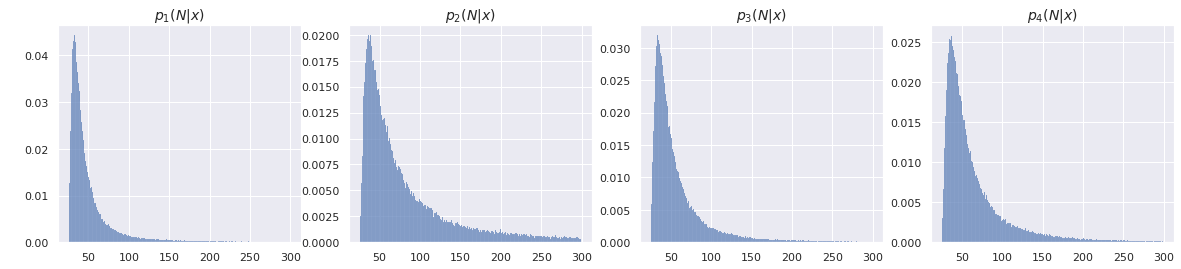
\includegraphics[width=\textwidth]{../../images/marginal-distributions.png}
    \caption{Marginal posterior distributions of $N$ for models Raftery, uninformative, geometric independent, and geometric dependent, respectively, for Waterbuck data set.}
    \label{fig:marginal-posteriors}
\end{figure}

\begin{table}[!ht]
    \centering
    \begin{tabular}{|c|c|c|c|c|}
        \hline
        {\bf Models} & {\bf Mean} &  {\bf Median} &   {\bf MRSE} &
        {\bf HDI} \\\hline
        {\bf Raftery} &   88.98 &   40.65 &  37.88 &  [26.00, 124.75] \\\hline
        {\bf Uninformative} &  856.54 &   67.41	 &  47.37 &   [26.01, 561.02] \\\hline
        {\bf Geometric independent} &   65.98 &   46.70 &  41.39 &  [26.02, 137.34] \\\hline
        {\bf Geometric correlated} &    72.44 &   51.82 &  44.01 &    [26.04, 161.18] \\\hline
        \end{tabular}
        \caption{Point estimates and highest density interval for each model in Impala data set.}
        \label{tab:summary-statistics-posterior-impala}
\end{table}

\begin{figure}[!ht]
    \centering
    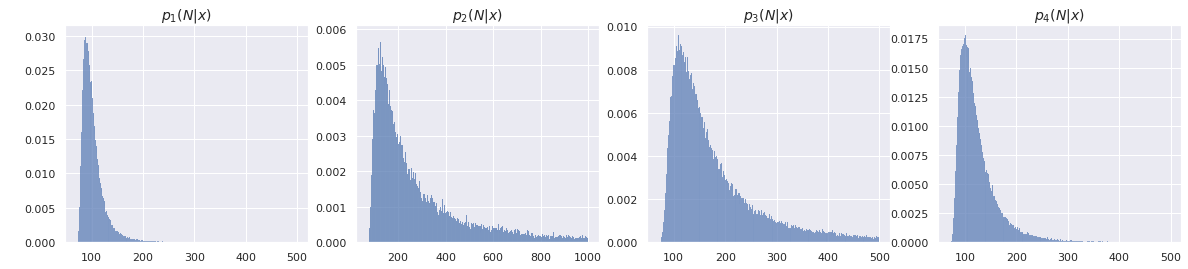
\includegraphics[width=\textwidth]{../../images/marginal-distributions-waterbuck.png}
    \caption{Marginal posterior distributions of $N$ for models Raftery, uninformative, geometric independent, and geometric dependent, respectively, for Waterbuck data set.}
    \label{fig:marginal-posteriors-waterbuck}
\end{figure}

\begin{table}[!ht]
    \centering
    \begin{tabular}{|c|c|c|c|c|}
        \hline
        {\bf Models} &     {\bf Mean} &  {\bf Median} &    {\bf MRSE} &    {\bf HDI} \\\hline
        {\bf Raftery} &   104.98 &   97.19 &   96.68 &  [74.74, 143.35] \\\hline
        {\bf Uninformative} &  1111.69 &  235.74 &  155.66 &  [75.0, 1920.81] \\\hline
        {\bf Geometric independent} &   221.70 &  154.46 &  132.79 &  [75.08, 470.09] \\\hline
        {\bf Geometric correlated} &   220.72 &  166.26 &  140.25 &  [78.86, 476.56] \\\hline
    \end{tabular}
    \caption{Point estimates and highest density interval for each model in Waterbuck data set.}
    \label{tab:summary-statistics-posterior-waterbuck}      
\end{table}

    In order to see if the real approximation used in Stan is good for the
    discrete parameter $N$, we compare the sample generated with the closed-form distributions
    (up to a constant) geometric independent and uninformative. To calculate
    the constant, we sum the values until we reach the zero from {\it NumPy}.
    From figure \ref{fig:approximation-stan}, we note that the approximation
    is good, even though for the uninformative model,
    both suffer from numerical issues.  Because of this we follow with this
    approach. 

\begin{figure}[!ht]
    \centering
    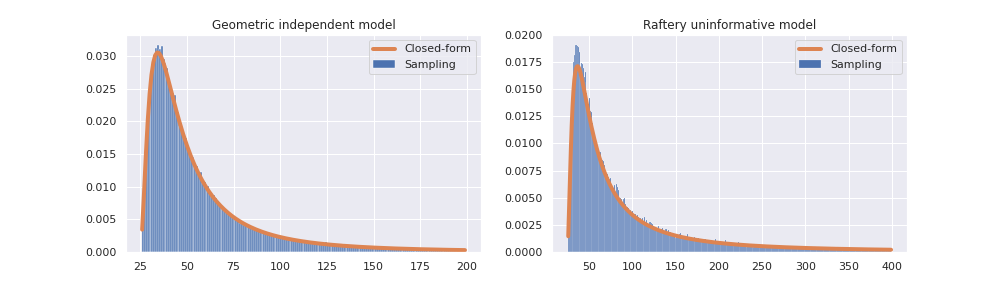
\includegraphics[width=\textwidth]{../../images/approximation-analysis-stan.png"}
    \caption{Approximation analysis of Stan's assumption that $N$ is a positive real number. }
    \label{fig:approximation-stan}
\end{figure}